\section{Evaluation}
\label{sec:evaluation}

We evaluate five questions:
\begin{enumerate}[leftmargin=*,itemsep=0pt,topsep=2pt,label=\textbf{Q\arabic*:}]
  \item Does the cross-partition pipeline preserve application semantics?
  \item Why must dependency and transport be measured as a scheduling
  contract rather than a copy constant?
  \item Does \sys meet a frozen deadline in the formal campaign, and how does
  it compare with executable baselines?
  \item Are the tail and thermal results stable across independent sessions?
  \item How do confidence-bounded deadline misses and background goodput
  change with offered load?
\end{enumerate}

\subsection{Experimental Setup}

\textbf{Evidence status.}
A thermal-normalized formal campaign is now bound to the frozen workload,
runtime, arrival trace, and promotion rules described below.

\textbf{Platform.}
All promoted measurements run on one Jetson AGX Thor using a fixed 1g+2g MIG
layout.  The 1g producer exposes eight SMs and shares a private MPS server with
the best-effort tenant; the 2g consumer exposes twelve SMs.  The software stack
is Jetson Linux R39.2, CUDA 13.2, and TensorRT 10.16.2.  Frequencies, process
placement, MIG UUIDs, quotas, and required thermal sensors are frozen by the
campaign manifest.

\textbf{Primary workload.}
The formal workload is a real ResNet-50 ImageNette classifier.  The backbone
runs on 1g and emits the $[1,1024,14,14]$ FP32 tensor described in
\S\ref{sec:implementation}; its trained head runs on 2g.  DistilBERT-SST2
generates best-effort load on 1g at a predeclared open-loop period.  Each
treatment consumes the same request-input trace, \texttt{JDGARR1} operational
release trace, engines, class map, and output oracle.

\textbf{Additional applications and controls.}
We use a real Whisper-Tiny encoder/decoder path on LibriSpeech dev-clean to
test ASR semantics.  A learned ResNet10 backbone/head split supplies the
same-activation causal and transport controls.  The latter is deliberately
not folded into the ImageNette SLO campaign because it has a different model,
payload, and evidence scope.

\textbf{Deadline and sessions.}
Two 1,100-request calibration blocks produce a pooled
$2{,}050.439~\mu$s p99.  Applying the predeclared 1.10 factor freezes
$D=2{,}255.483~\mu$s before treatment execution.  The formal campaign has six
counterbalanced sessions, 1,100 measured requests per system per session, and
6,600 requests per system.  Each session executes NVIDIA MPS, native XSched,
and \sys in one of the frozen balanced orders.  We use request-level samples
for pooled distributions and the six sessions as the statistical units for
paired treatment effects.

\textbf{Metrics and qualification.}
Production-wall latency is Equation~\ref{eq:production-wall}.  We report p50,
p99, p99.9, deadline misses, and completed best-effort requests/s.  Deadline
qualification uses the exact one-sided 95\% Clopper--Pearson upper bound
(CP95) on deadline-miss ratio (DMR), with target $\epsilon=0.0005$.
Zero observed misses are not alone sufficient: the sample count must make
CP95 no greater than $\epsilon$.  All percentiles are Type~7 and replayed from
request-level CSV files.

\subsection{Q1: Application Semantics}

\PnineApplicationTable

Table~\ref{tab:application-gates} reports the two application gates.
ImageNette uses 100 labelled inputs, with ten warmup and 90 measured requests.
The unsplit reference and cross-partition candidate both reach 0.8333
classification accuracy, above the frozen 0.80 threshold, with zero accuracy
delta.  The gate binds each image digest to the external label and records
independent reference and candidate output containers.

Whisper uses twelve LibriSpeech dev-clean utterances, with two warmup and ten
measured requests.  Reference and candidate both reach 0.9000 utterance
exact-match accuracy and 0.1127 WER, below the frozen 0.20 maximum.  Their
complete output containers have the same SHA-256 digest, not merely the same
aggregate score.  Thus, the 2.304-MB activation edge preserves the decoder's
observable transcript for every recorded input.

The thermal campaign repeats a fixed ImageNette trace at greater scale.  All
three systems attain 0.8345 accuracy with zero candidate/reference delta in
every session.  Consequently, the SLO differences below cannot be attributed
to dropping requests from the accuracy calculation or weakening the oracle.

\subsection{Q2: Dependency Changes Contention, Not Only Copy Time}

\begin{figure*}[t]
  \centering
  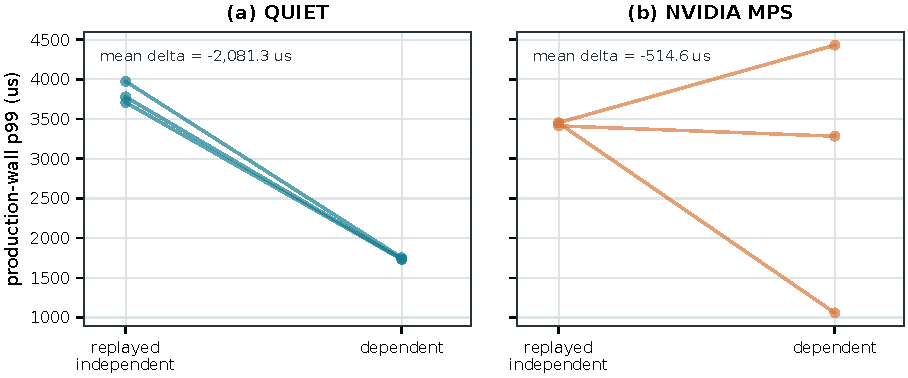
\includegraphics[width=\textwidth]{figures/p9-causal-pairs.pdf}
  \caption{Exploratory same-activation causal replay on the learned ResNet10
  split.  Each line is one sequential pair with 20 measured requests per arm;
  dependent minus independent is the signed effect.  \sys has mean
  $-2{,}081.286~\mu$s (95\% paired-session interval
  $[-2{,}394.953,-1{,}767.619]~\mu$s).  NVIDIA MPS has mean
  $-514.579~\mu$s and an interval spanning zero.  The experiment is not
  thermal normalized and supports a mechanism claim only.}
  \Description{Two paired-line plots compare replayed-independent and
  dependent p99 latency over three repeats for QUIET and NVIDIA MPS.}
  \label{fig:causal}
\end{figure*}

The replayed independent arm binds the request's pre-captured producer
activation before release and permits producer and consumer execution to
overlap.  The dependent arm releases the consumer only after live publication.
All other inputs remain equal.  If the edge were merely an additive copy
penalty, the dependent arm should differ by a stable positive offset.

Figure~\ref{fig:causal} shows the opposite for \sys: serializing on publication
reduces p99 by $1{,}977.575$--$2{,}221.892~\mu$s across all three pairs.
Concurrent independent execution increases shared-SoC contention enough to
outweigh the waiting it removes.  MPS is unstable across pairs: its signed
effects are $+977.388$, $-2{,}391.266$, and
$-129.859~\mu$s, yielding a wide interval that includes zero.  The result
does not claim that dependencies intrinsically improve latency.  It shows
that precedence selects a contention schedule and must therefore be explicit
in the runtime.

A separate 20-request transport control reinforces this point.  For the
1,884,160-byte learned detector edge, registered direct binding has
$2{,}195.508~\mu$s edge p99 and $2{,}908.268~\mu$s wall p99.  Pinned bounce
has a lower $1{,}863.770~\mu$s edge p99 and
$2{,}538.617~\mu$s wall p99, while pageable bounce reaches
$2{,}283.200~\mu$s and $2{,}975.838~\mu$s, respectively.  All three emit the
same output trace.  Notification dominates the registered case in this short
run, whereas copies dominate the pageable case.  Because the experiment is
small and nonthermal, we use it to reject a universal
\emph{registered-is-fastest} assumption, not to rank transports.  \sys instead
profiles the joint tail selected by Equation~\ref{eq:joint-tail}.

\subsection{Q3: Thermal-Normalized Deadline Performance}

\PnineFormalTable

\begin{figure*}[t]
  \centering
  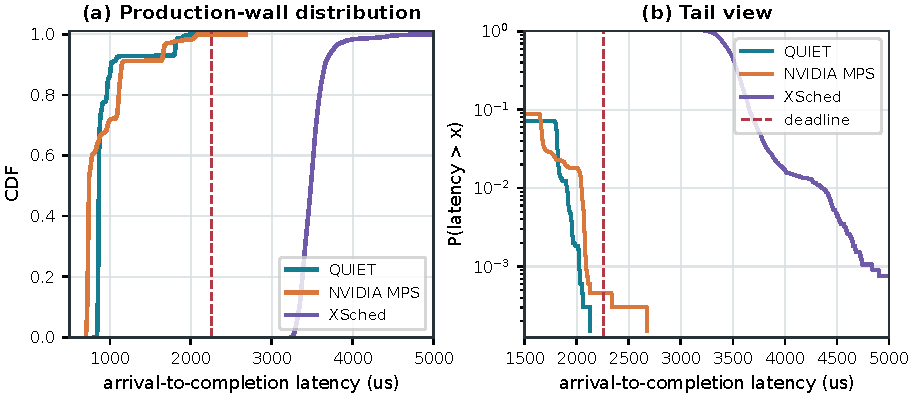
\includegraphics[width=\textwidth]{figures/p9-latency-cdf.pdf}
  \caption{Request-level latency in the six-session thermal-normalized
  ImageNette campaign (6,600 requests/system).  The left panel shows the full
  CDF; the right isolates the tail on a logarithmic survival axis.  The dashed
  line is the frozen $2{,}255.483~\mu$s production-wall deadline.}
  \Description{Two plots compare QUIET, NVIDIA MPS, and XSched latency.  QUIET
  and MPS lie mostly left of the deadline; the XSched distribution lies to its
  right.  The logarithmic tail reveals two MPS misses and no QUIET miss.}
  \label{fig:latency-cdf}
\end{figure*}

Table~\ref{tab:formal-campaign} and Figure~\ref{fig:latency-cdf} give the
formal result.  \sys completes all 6,600 requests before the deadline.  Its
p50, p99, and p99.9 are $863.886$, $1{,}902.987$, and
$2{,}025.643~\mu$s.  The zero-miss CP95 bound is 0.0454\%, which qualifies
for the 0.05\% target.

NVIDIA MPS has a lower $739.887~\mu$s median but a
$2{,}045.606~\mu$s p99 and incurs two deadline misses.  Its observed DMR is
0.0303\%, yet CP95 is 0.0954\%; it therefore does not qualify.  This gap
between median and tail is precisely the behavior that a fixed spatial share
does not expose to a dependent request.  \sys narrows the protected interval
without surrendering the producer tail.

The native XSched port misses all 6,600 requests.  Its median is
$3{,}484.202~\mu$s, and its p99 is $4{,}351.332~\mu$s.  Output accuracy remains
0.8345 with zero delta, so the row is a valid execution of the application but
is infeasible at this lock.  We report the failure rather than retune the
deadline or relabel a local approximation as XSched.

Background throughput separates tail protection from capacity destruction.
\sys completes 249.909 best-effort requests/s, NVIDIA MPS completes 249.941,
and XSched completes 97.845.  Across the six paired sessions, the \sys-minus-MPS
p99 effect is $-138.508~\mu$s with 95\% interval
$[-233.217,-43.798]~\mu$s.  The paired goodput effect is
$-0.0317$ requests/s with interval $[-0.0988,0.0354]$, which does not resolve
a directional difference.  Thus, the supported claim is a tail reduction at
statistically indistinguishable background goodput, not a throughput gain.

\subsection{Q4: Session and Thermal Stability}

\begin{figure*}[t]
  \centering
  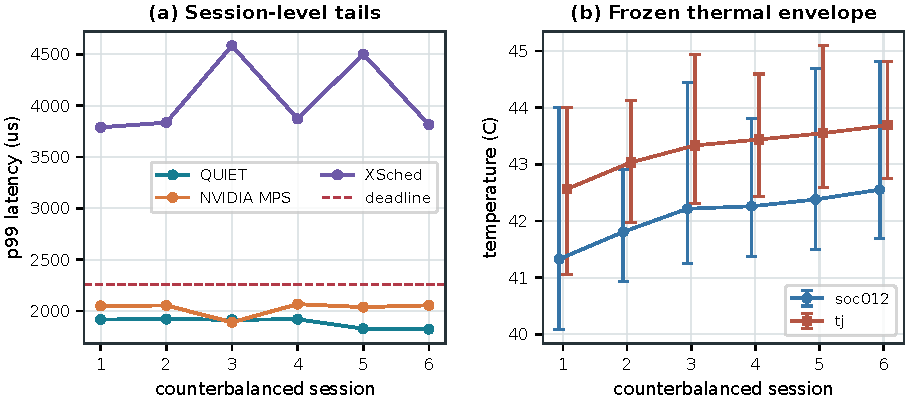
\includegraphics[width=\textwidth]{figures/p9-session-stability.pdf}
  \caption{Independent-session stability.  Panel (a) reports each session's
  p99 against the fixed deadline.  Panel (b) reports mean \texttt{soc012} and
  \texttt{tj} temperatures with observed minimum--maximum bars.  Thermal
  conditions define admissibility; they are not used to rescale latency.}
  \Description{The left plot shows six session p99 values for QUIET, MPS, and
  XSched against the deadline.  The right shows soc012 and tj means with
  observed temperature ranges for the same sessions.}
  \label{fig:stability}
\end{figure*}

Figure~\ref{fig:stability}(a) shows that all six \sys session p99s remain below
$1{,}921~\mu$s.  MPS is also below the deadline at session-p99 granularity,
but its two request-level misses prevent confidence qualification.  XSched is
above the deadline in every session.  The counterbalanced order prevents one
treatment from consistently receiving the first or last thermal position.

Each session contains 430--434 \texttt{tegrastats} samples.  The largest
within-session \texttt{soc012} range is $3.907^\circ$C and the largest
\texttt{tj} range is $2.938^\circ$C, both below the frozen
$8^\circ$C limit.  Cross-session mean temperature changes by at most
$0.910^\circ$C, below the $4^\circ$C envelope, and every sample set contains
the required VDD\_GPU rail.  Figure~\ref{fig:stability}(b) also makes the
slow drift visible rather than hiding it behind an aggregate mean.  The gate
accepts this envelope but does not claim identical temperature.

\subsection{Q5: DMR--Goodput Frontier}

\begin{figure*}[t]
  \centering
  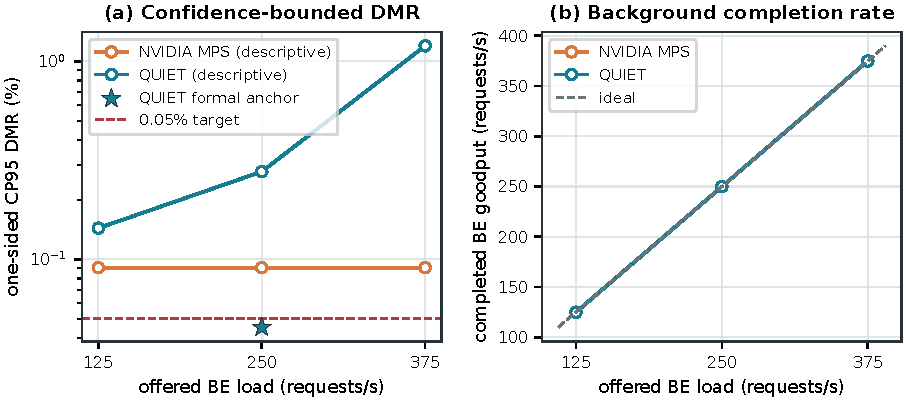
\includegraphics[width=\textwidth]{figures/p9-load-frontier.pdf}
  \caption{Same-workload offered-load sweep.  Hollow markers are descriptive
  three-session points (3,300 requests/point) and are not thermal normalized.
  The star is the separate six-session, thermal-qualified \sys anchor at
  250 requests/s.  No hollow point is used for ranking.}
  \Description{The left log-scale plot shows CP95 deadline-miss bounds versus
  offered load and a qualified QUIET star below the target.  The right plot
  shows QUIET and MPS goodput closely following the ideal line.}
  \label{fig:load-frontier}
\end{figure*}

Figure~\ref{fig:load-frontier} varies best-effort load.  At 125, 250, and
375 offered requests/s, \sys completes 124.941, 249.908, and 374.897 rps.
MPS completes 124.950, 249.888, and 374.868 rps.  Both track the ideal line,
so goodput alone makes them appear indistinguishable.

Confidence-bounded DMR exposes a different picture.  MPS observes no misses at
all three points, but 3,300 requests only bound DMR by 0.0907\%, above the
0.05\% target.  \sys observes 1, 4, and 29 misses, producing CP95 bounds of
0.1437\%, 0.2772\%, and 1.1963\%.  The 375-request/s point also exceeds the
selected plan's gate bound.  These points describe overload behavior; the
campaign's \sys star is the only statistically qualified point because it has
6,600 thermally admitted requests and zero misses.  We do not combine the
three-session 250-request/s point with that anchor because their session and
thermal contracts differ.

\subsection{Executed Comparator Coverage}

\PnineComparatorTable

Table~\ref{tab:native-comparators} includes every comparison implementation
that executed locally.  Evidence class A is the directly ranked formal
campaign: XSched's native path participates in that campaign and is infeasible
at the frozen deadline.  Pantheon is class B: its pinned online scheduler,
priority tiers, and model chunks preserve 0.8333 accuracy on the 90-request
ImageNette gate, with two misses and a $4{,}133~\mu$s p99.  Its protobuf
interface floors a distinct $2{,}224.448~\mu$s deadline to integer
microseconds, so its number remains visible but is not pooled with
Table~\ref{tab:formal-campaign}.

Orion is also shown rather than omitted.  Its ImageNette port preserves 0.8333
accuracy.  Under its separate diagnostic contract
($D=5{,}722.576~\mu\mathrm{s}$), it records zero misses and reaches a
$5{,}537.090~\mu$s p99.  The earlier balanced Whisper campaign additionally
records zero misses over 9,000 requests, a
$1{,}569.738~\mu$s p99, and 153.571 background requests/s.  These are scoped
numeric results, not a formal rank, because the upstream differential
scheduler trace is incomplete and the older campaign is nonthermal.

The remaining rows expose measured mechanism boundaries.  NVIDIA MIG, GSLICE,
and gpulet retain their raw-replayed historical numbers.  BLESS executes its
affinity scheduler and q25 switch boundary but cannot deserialize the exact
q100 plan in the required restricted context.  BOER and ParvaGPU pass numeric
independent-service controls before rejecting or failing the dependent
contract.  DeepPlan selects direct host access from the measured transport
profile.  Thus, a failed common-contract gate changes the evidence class; it
does not erase an experiment that ran.

\subsection{Limitations}

Our strongest claim is deliberately narrow: one Thor device, a fixed 1g+2g
placement, one thermal envelope, and a two-stage ImageNette chain.  The
production path is low-inflight; the validated three-slot ring has not yet
carried the formal TensorRT workload.  The ASR gate establishes application
semantics on ten measured utterances but is not a thermal SLO campaign.  The
causal, transport, and load-sweep results remain exploratory or descriptive as
marked.  Every locally executed comparator appears in
Table~\ref{tab:native-comparators}, while only its class-A rows support direct
same-condition ranking.

\sys also depends on coherent integrated memory and cooperative pause
acknowledgement.  Its current boundary does not preempt a running kernel, and
its results do not transfer automatically to discrete GPUs or larger
multi-stage DAGs.  These limitations constrain generality, but they do not
alter the formal result inside the frozen contract.
